\documentclass[aspectratio=169]{beamer}

\usepackage[utf8]{inputenc}
%\usepackage{latexsym}
\usepackage{graphicx}
\usepackage{mathptmx}
\usepackage{amsmath}
%\usepackage{amsfonts}
\usepackage{amssymb}
\usepackage{amsbsy}
\usepackage{amsthm}
\usepackage{algorithmic}

% Fancy figures
\usepackage{multicol}
\usepackage{subcaption}

% Tikz
\usepackage{tikz}
\usetikzlibrary{arrows.meta, positioning}

% Get checkmark logo
\usepackage{pifont}
\newcommand{\cmark}{\ding{51}}
\newcommand{\xmark}{\ding{55}}
% Get \lee and \gee commands
\newcommand{\lee}{\leqq}
\newcommand{\gee}{\geqq}

% Strikouts
\usepackage[normalem]{ulem}

% Restore Mathcal
\let\saveboldmath\boldmath
\usepackage{mathptmx}
\let\boldmath\saveboldmath
\usepackage{bm}
\DeclareSymbolFont{cmsymbols}{OMS}{cmsy}{m}{n}
\SetSymbolFont{cmsymbols}{bold}{OMS}{cmsy}{b}{n}
\DeclareSymbolFontAlphabet{\mathcal}{cmsymbols}

\include{header}
% Title Information
\title{Leveraging Interpolation Models and Error Bounds for Verifiable Scientific Machine Learning}
\subtitle{
Journal of Computational Physics 524, Article 113726 (2025).
\url{doi.org/10.1016/j.jcp.2025.113726}
}
\author{Tyler Chang$^{1,4}$, Andrew Gillette$^2$, and Romit Maulik$^{1,3}$}
\date{Presentation at SIAM NCC 2025\\October 26, 2025}
\institute{Argonne$^1$, Lawrence Livermore$^2$, Penn State$^3$, Siemens EDA$^4$}

\begin{document}

% Title slide
\setbeamertemplate{footline}{}
{
    \frame{\titlepage}
}

% Begin body
\setbeamertemplate{footline}[page number]{}

\section{Introduction and SciML Context}

% Slide 1: AI, SciML, and Interpolation
\begin{frame}
\frametitle{AI, SciML, and Interpolation}
    AI = {\sl Representation Learning} + {\sl Regression/Interpolation}

    \begin{center}
    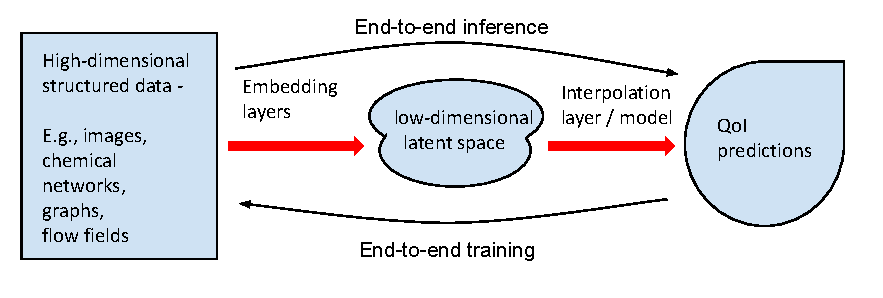
\includegraphics[width=0.9\textwidth]
    {../img/delaunay_new/interpolating_latent_space.pdf}
    \end{center}

    SciML = {\bf separate} representation learning and regression or
    interpolation

    \medskip

    This paper = {\bf just interpolation} in the context of SciML
\end{frame}

% FRAME: overview of remaining paper
\begin{frame}
\frametitle{Outlines}
    \tableofcontents
\end{frame}

\section{Interpolation Models and Error Bounds}

% Slide 2: Piecewise linear (Delaunay) interpolation
\begin{frame}
\frametitle{Piecewise Linear (Delaunay) Interpolation}

    Approximate $f(q)$ by piecewise linear ${\hat f}_T(q)$;
    $T$ = simplicial mesh
    \begin{center}
    \includegraphics[width=0.25\textwidth]
    {../img/delaunay_new/inference_1d_pt3.eps}
    $\qquad\quad$
    
\includegraphics[width=0.25\textwidth]
    {../img/delaunay_old/seamount.eps}\\
    {\small
    1 dimension
    $\qquad\qquad\qquad\quad$
    $d$ dimensions
    }
    \end{center}

    If $S \in T$ contain $q$ $\quad;\quad$ diameter$(S) = h$:
    $$
    |f(q) - {\hat f}_{T}(q)| \leq
    \left(\frac{\gamma + \gamma\sigma\sqrt{d}}{2}\right)h^2
    $$
    {\small
    $\gamma$ = Lip const of $\nabla f$;
    $\sigma$ = condition number of interpolation matrix (skew of $S$);
    % $\sigma$ can often be bounded if we use $T = DT$
    }
\end{frame}

% Slide 3: RBF (thin-plate spline) interpolation
\begin{frame}
\frametitle{RBF Interpolation (thin-plate spline kernel)}

    Approximate $f(q)$ by ${\hat f}_{RBF}(q)$ = linear combination of radial
    basis functions (RBFs)

    \begin{center}
    ${\hat f}(q) =$
    $w_1$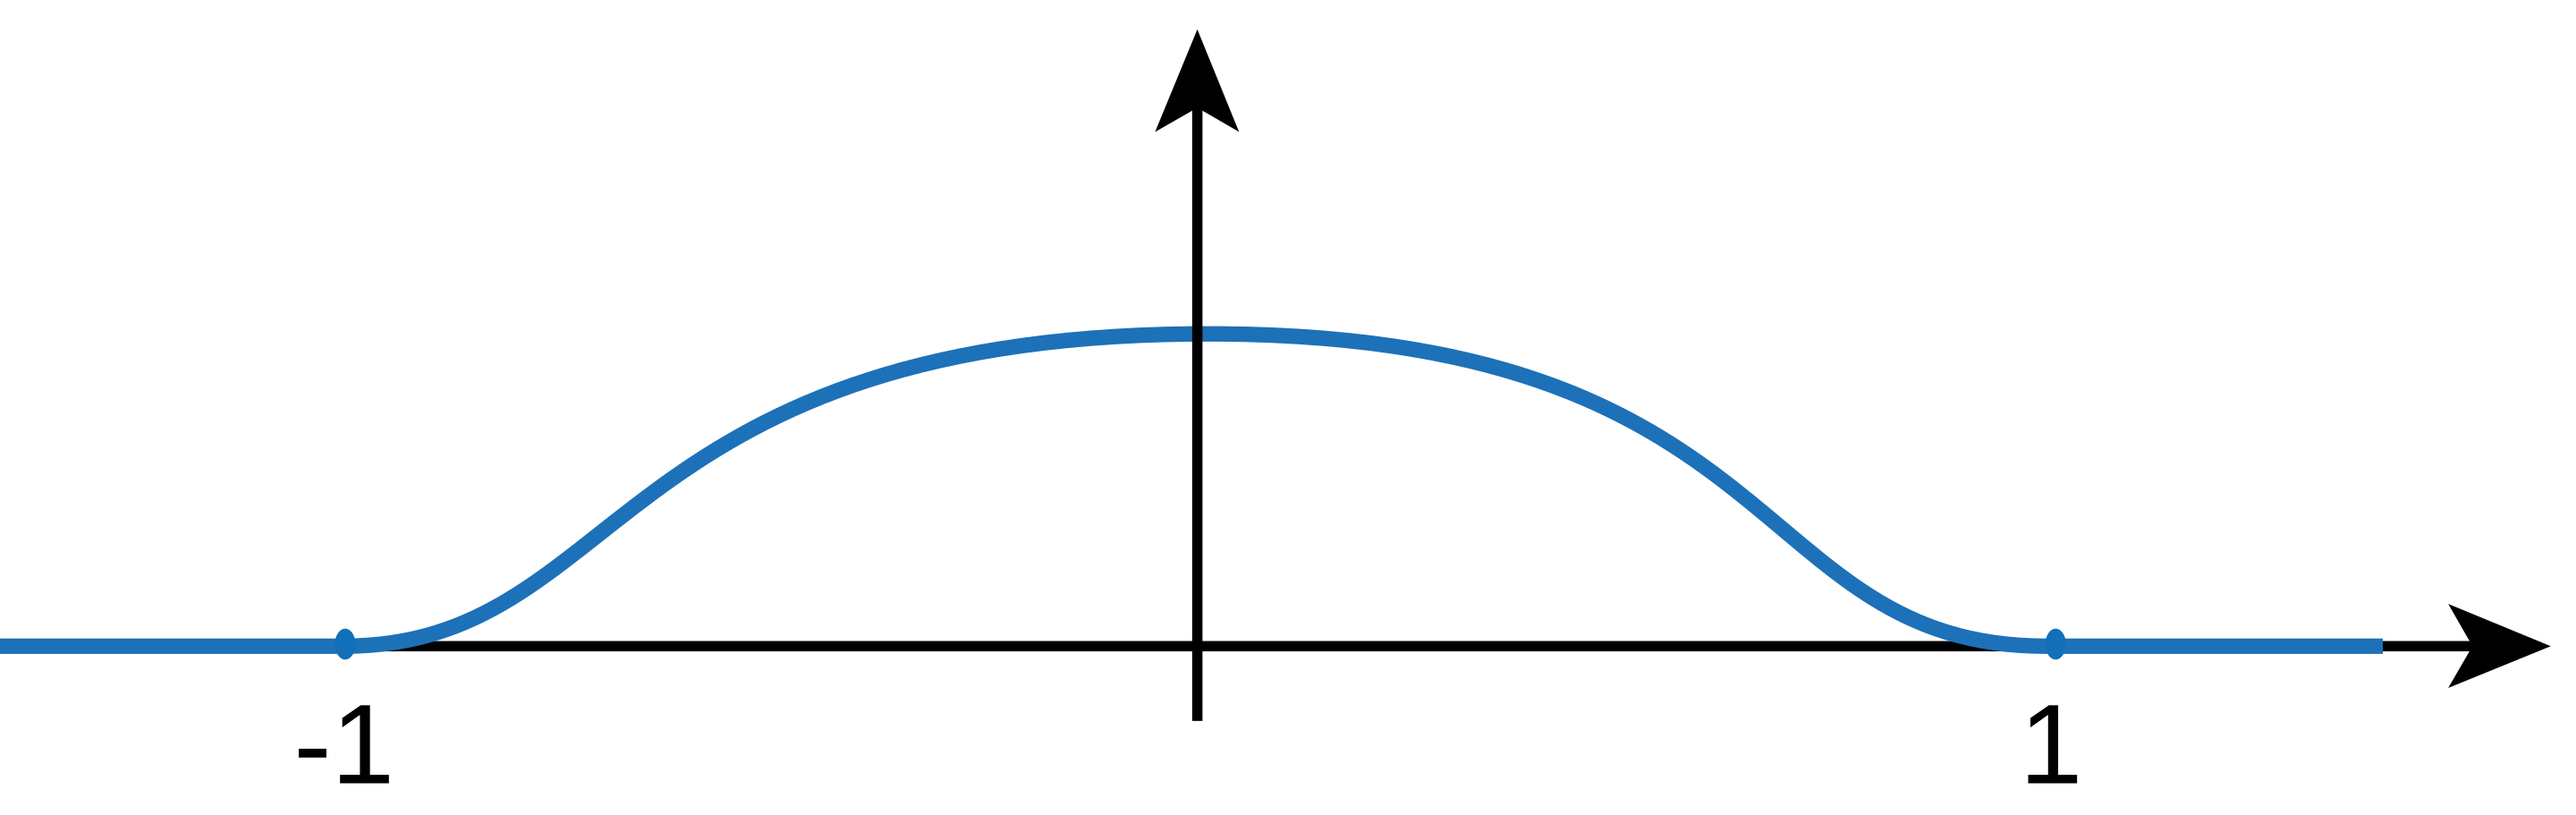
\includegraphics[width=0.1\textwidth]
    {../img/delaunay_new/bump.png} + 
    $w_2$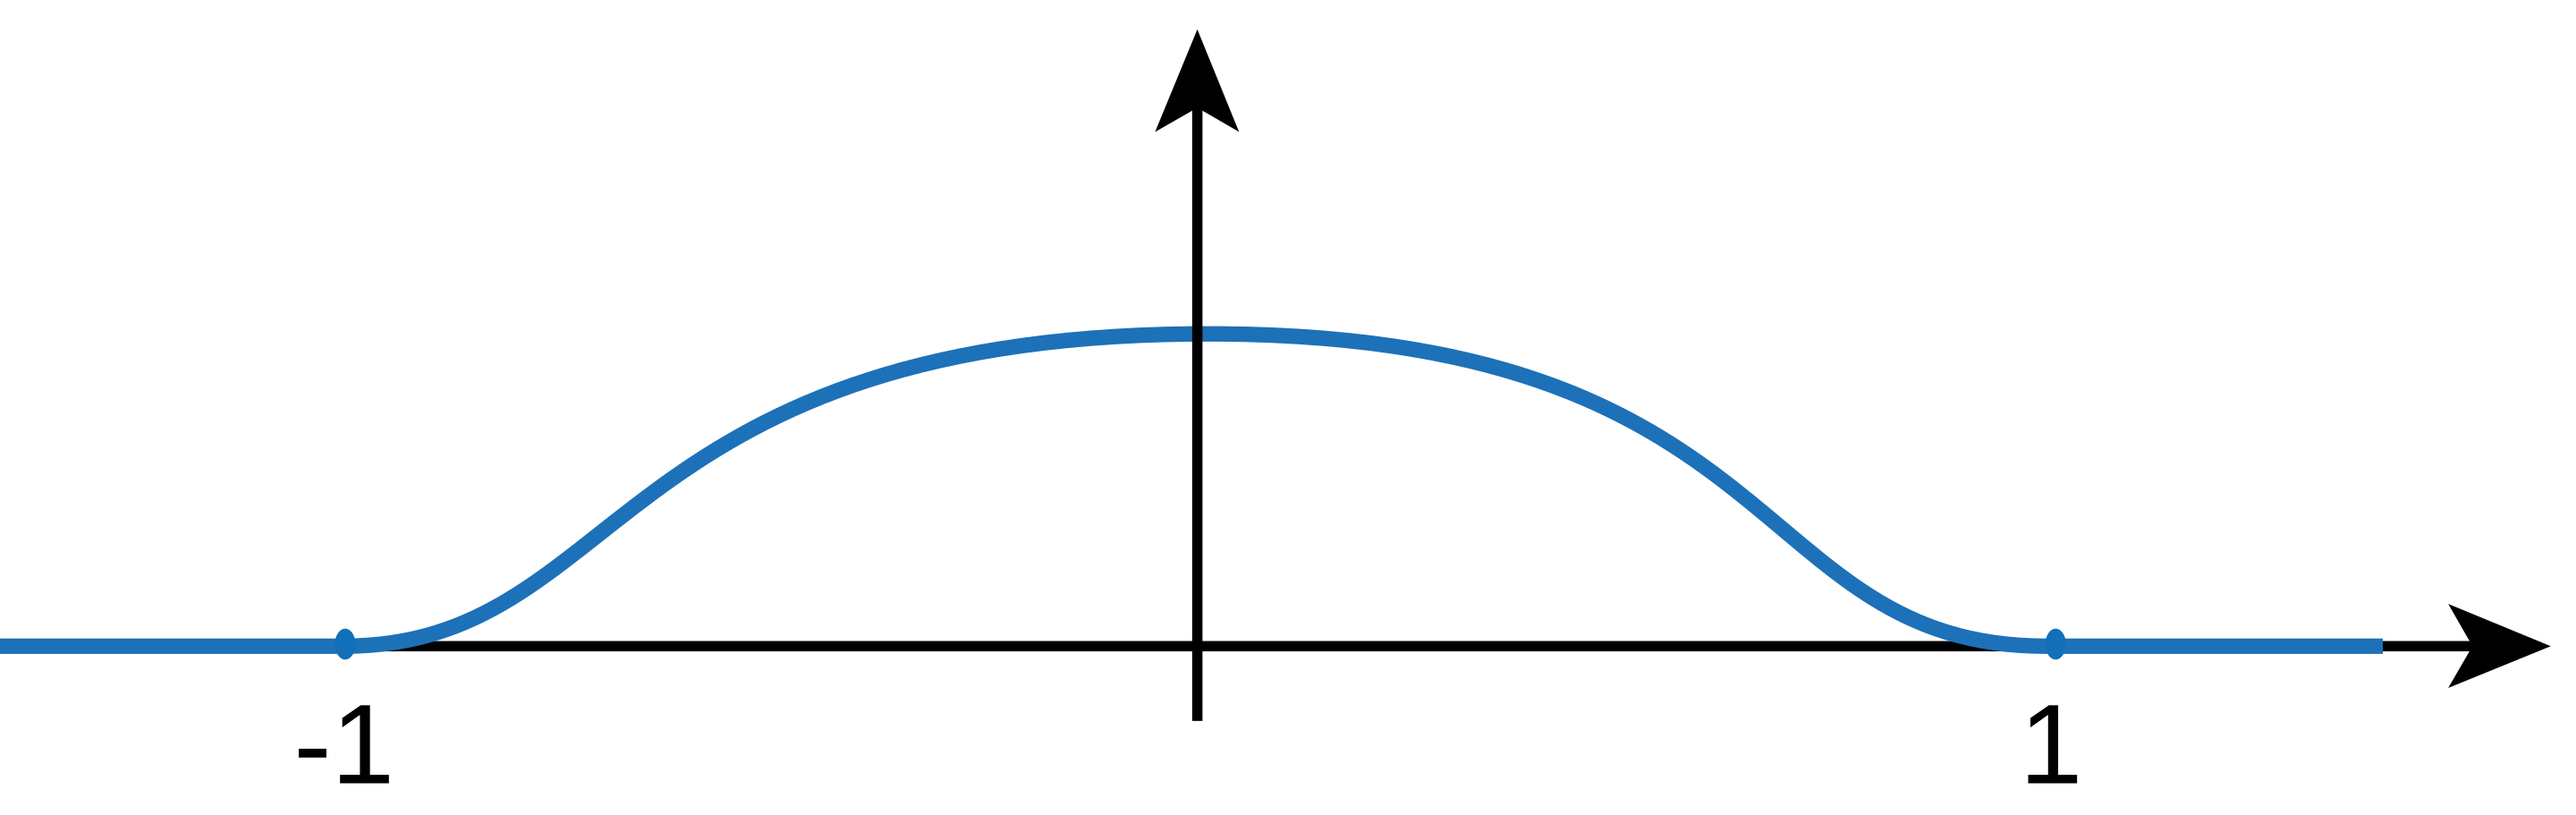
\includegraphics[width=0.1\textwidth]
    {../img/delaunay_new/bump.png} +
    $\ldots$ +
    $w_n$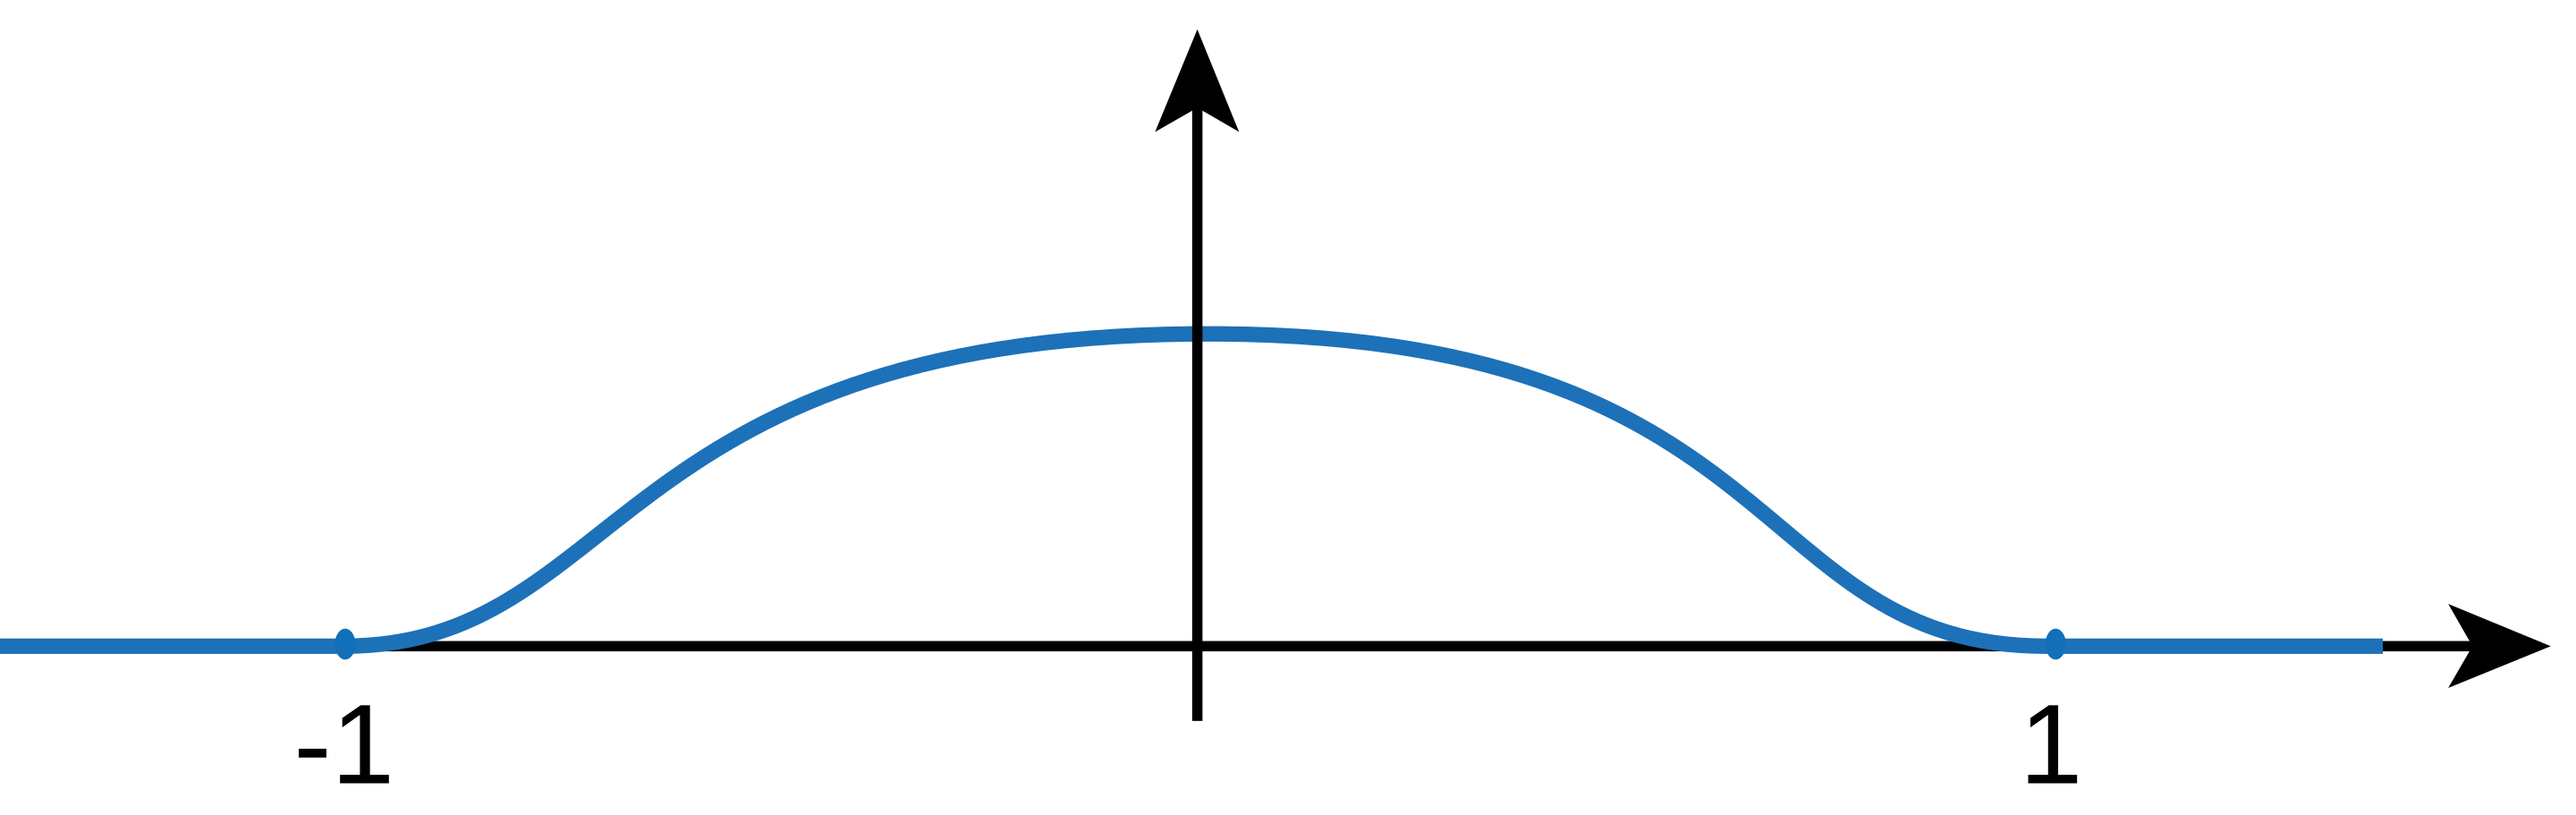
\includegraphics[width=0.1\textwidth]
    {../img/delaunay_new/bump.png} +
    {\sl tail}(q)
    \end{center}

    We use RBF = thin-plate-spline (TPS) in this work -- it is the default in
    SciPy

    \bigskip

    If $h$ = distance from $q$ to the nearest interpolation node (training
    point), then:
    $$
    |f(q) - {\hat f}_{RBF}(q)| \leq C \cdot h \sqrt{\log (h^{-1})}
    $$
    {\small
    $C$ is a constant depends on $f$, the choice of RBF, and (indirectly) on
    $d$, but independent of $h$
    }

    % {\bf Note:} as $h$ gets smaller, eventually the error gets {\sl worse} as
    % $\sqrt{\log (h^{-1})} \rightarrow \infty$
\end{frame}

% Slide 4: Gaussian process interpolation
\begin{frame}
\frametitle{Gaussian process interpolation}
    Two interpretations:
    \begin{enumerate}
    \item ${\hat f}_{GP}$ = RBF interpolant with ``Gaussian bump'' kernel
    \item ${\hat f}_{GP}$ = posterior distribution over all possible
        realizations of $f$ given the observations in the training data
    \end{enumerate}

    \bigskip

    (2) lets us use the variance of $q$ as an uncertainty heuristic:
    $$
    K(q, q) = \tau_f \left(
        1 - \| \phi^{(1)}(q), \ldots, \phi^{(1)}(q) \|_{A_{GP}^{-1}}^2 \right)
    $$
    {\small
    $\phi^{(1)}$, $\ldots$, $\phi^{(n)}$ are Gaussian basis functions;
    $\tau_f$ $\sim$ variance of $f$;
    $\| \cdot \|_{A_{GP}^{-1}}$ is a rescaling of $\|\cdot\|_2$
    }

    % {\bf Note:} as with the TPS RBF, as $h$ gets smaller, eventually the error
    % gets {\sl worse}.  This can be controlled by adjusting a shape parameter in
    % for each $\phi^{(k)}$
\end{frame}

% Slide 5: ANN/MLP models
\begin{frame}
\frametitle{Neural Network models (MLPs)}

    In a typical modern AI model:

    $${\hat f}_{ANN}(Q) = {\hat f}_{MLP} \circ {\hat f}_R(Q)$$
    where
    $${\hat f}_R(Q) : ? \rightarrow \mathbb{R}^d$$
    and
    $$
    {\hat f}_{MLP}(q) =
        \ell^{(N)} \circ \ell^{(N-1)} \circ \ldots \circ \ell^{(0)}(q)
    $$

    Each
    $$
    \ell^{(i)}(x^{(i)}) = u\left(W^{(i)}x^{(i)} + b^{(i)}\right)
    $$
    where $W^{(i)}$ and $b^{(i)}$ define a linear transformation, and $u$ is a
    nonlinear ``activation function''

    \bigskip

    We will focus on MLPs which use ReLU (piecewise linear) activation function
    which is the most common option
\end{frame}

\section{Experiments on Synthetic Data}

% Slide 6: Experiment setup
\begin{frame}
\frametitle{Experiments on synthetic datasets}
    For all the interpolation models we saw constants that depend on:
    \begin{enumerate}
        \item the dimension of the problem
        \item the density of the training data,
        \item the smoothness of $f$,
        \item the conditioning of the interpolation matrices,
    \end{enumerate}

    \medskip

    We generate hundreds of datasets from different distributions varying the
    \begin{enumerate}
        \item dimension $d$
        \item number of training points $n$
        \item Lipschitz constant of the underlying $f$
        \item skewness of the training points
    \end{enumerate}

    \medskip

    We use all methods on all training sets and measure the prediction
    errors on a holdout set generated from the same distribution.
\end{frame}

% Slide 7: Results for dimension/smoothness
\begin{frame}
\frametitle{Effects of problem dimension and smoothness}
    \begin{center}
    % Delaunay/MLP figure
    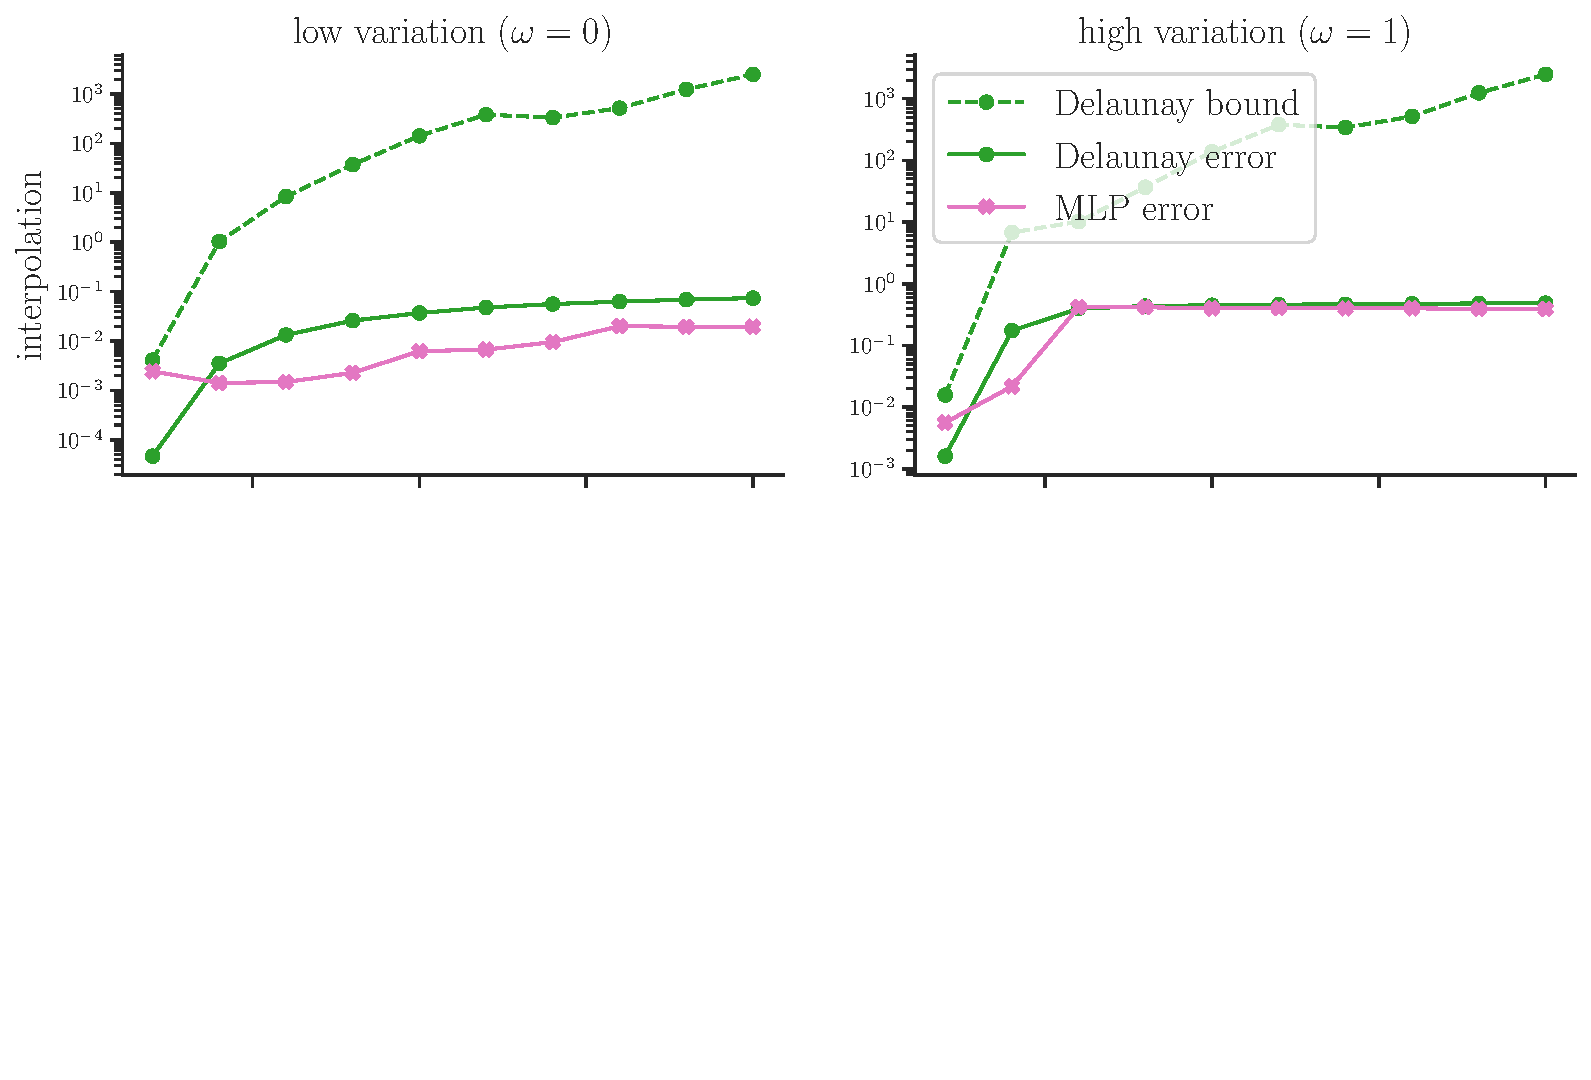
\includegraphics[width=0.75\textwidth]
    {../img/delaunay_new/del_mlp_dim_smooth_interp.pdf}\\

    % RBF/GP figure
    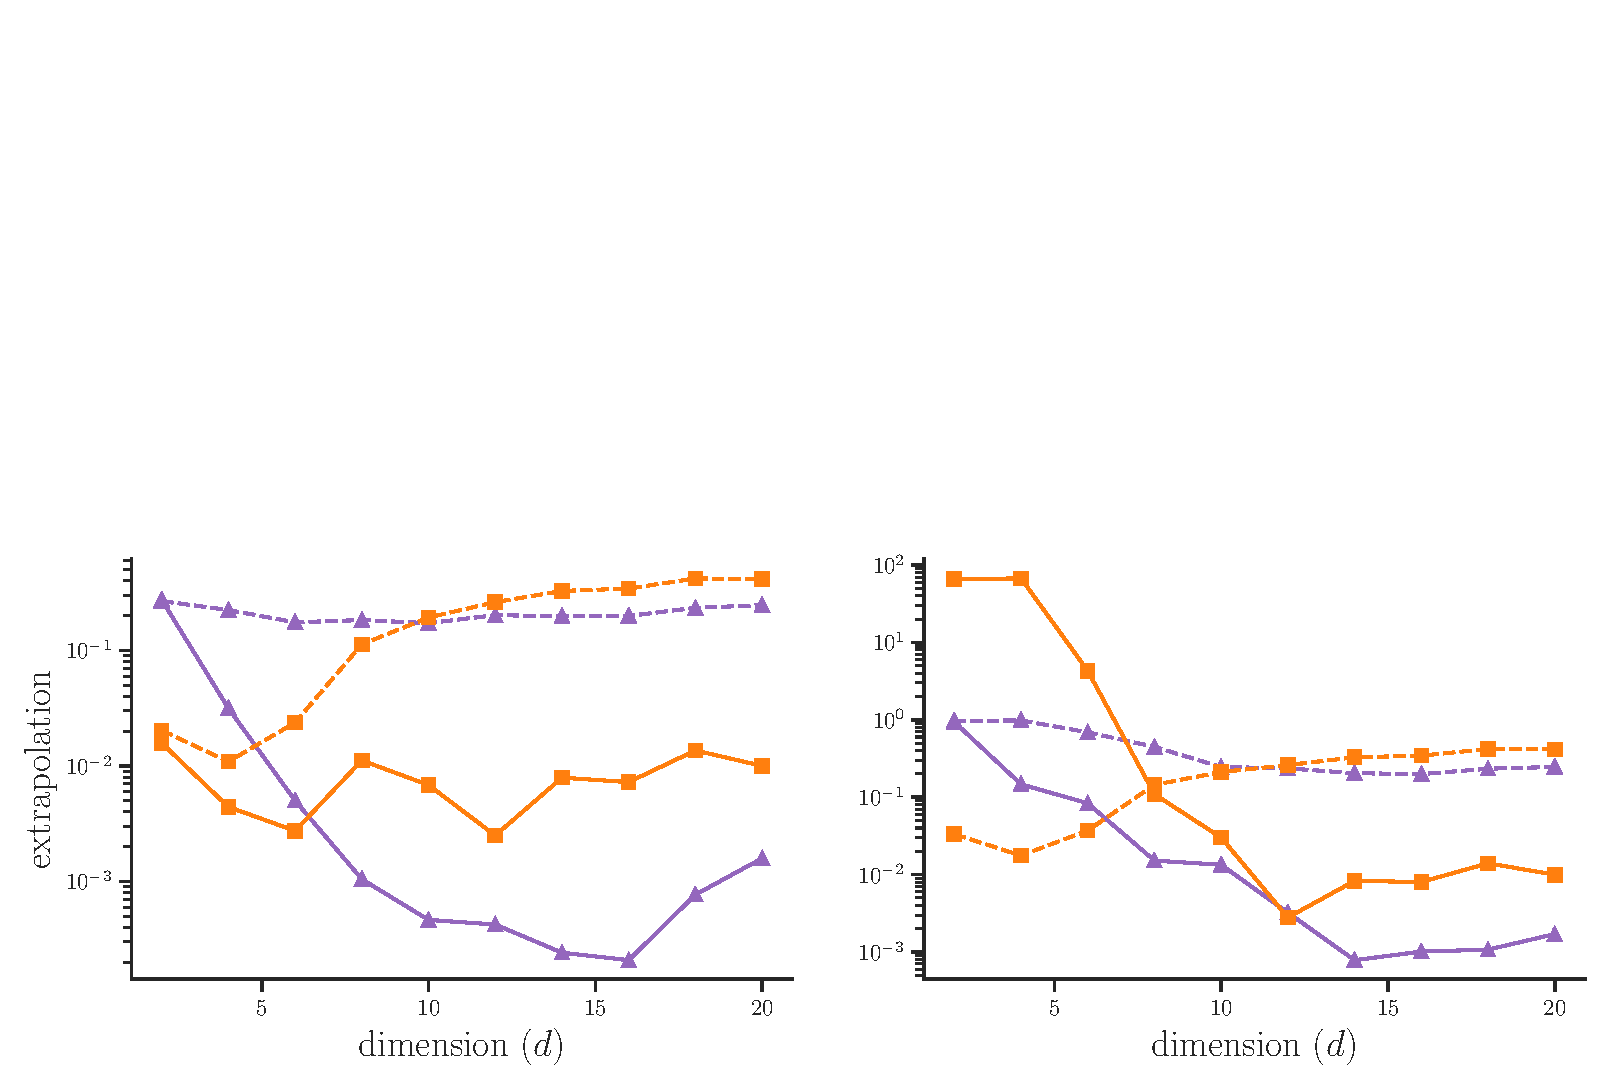
\includegraphics[width=0.75\textwidth]
    {../img/delaunay_new/rbf_gp_dim_smooth_extrap.pdf}
    \llap{%
        \raisebox{0.21in}{
        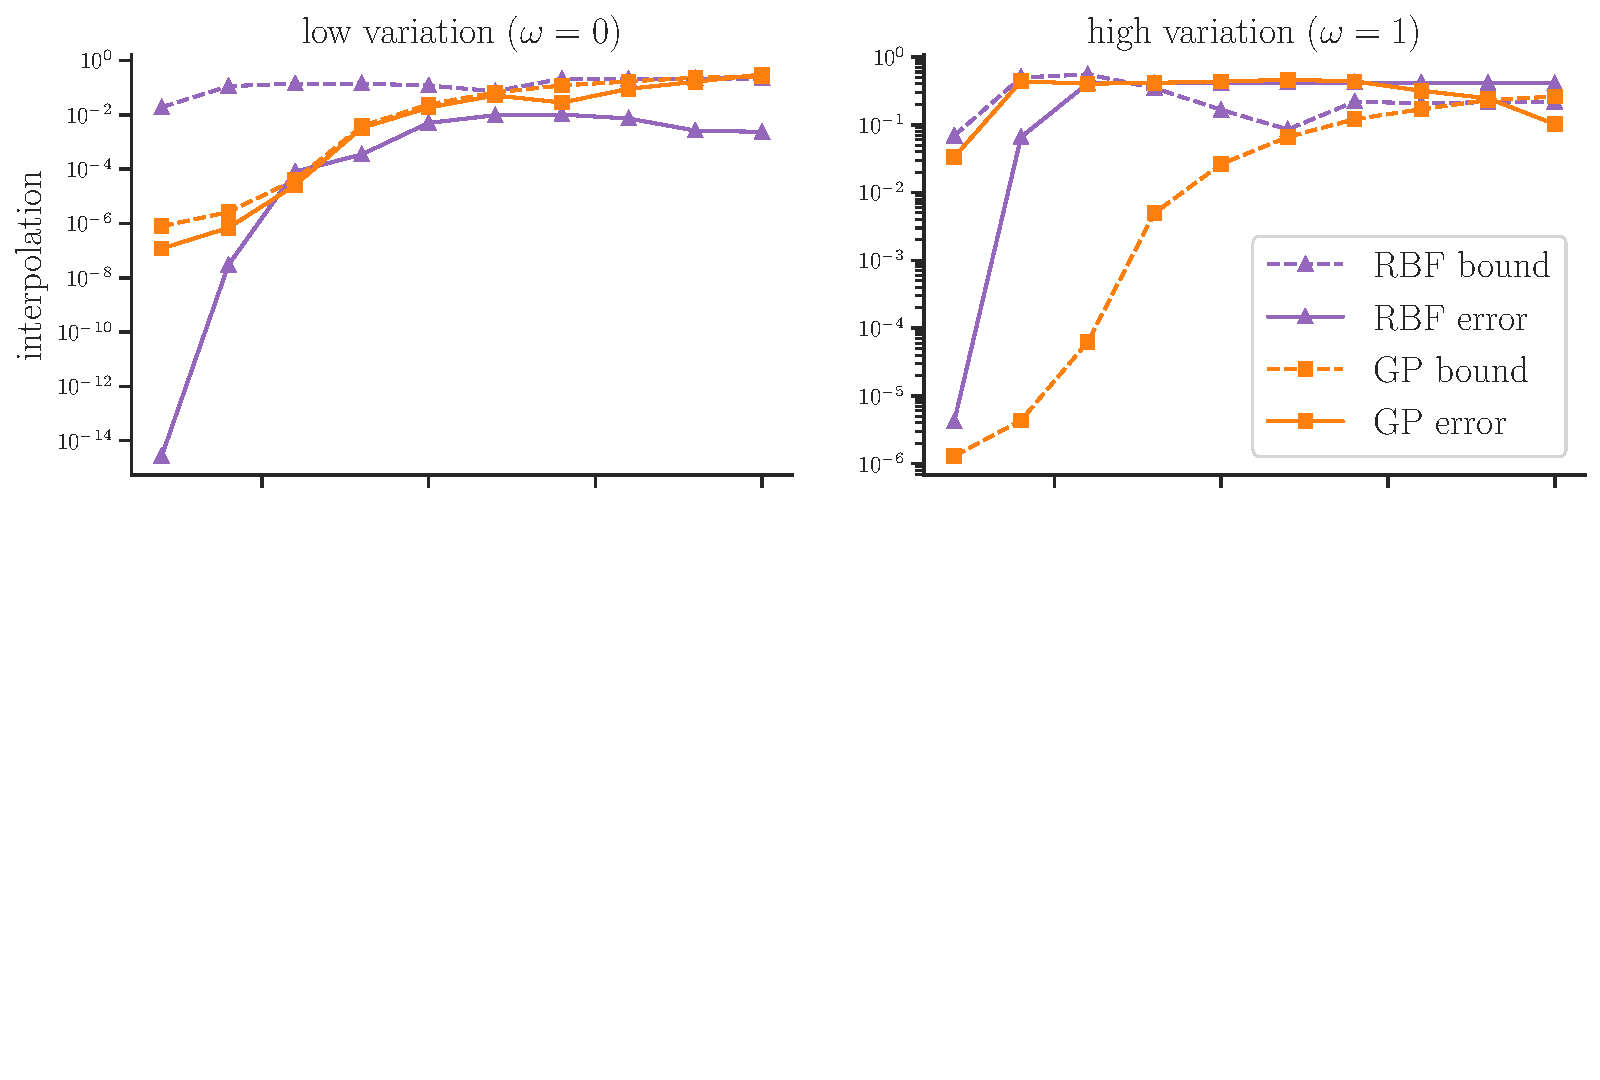
\includegraphics[width=0.75\textwidth]
        {../img/delaunay_new/rbf_gp_dim_smooth_interp.pdf}
        }%
    }
    \end{center}
\end{frame}

% Slide 8: Results for training sample size/smoothness
\begin{frame}
\frametitle{Effects of training sample size and problem smoothness}
    \begin{center}
    % Delaunay/MLP figure
    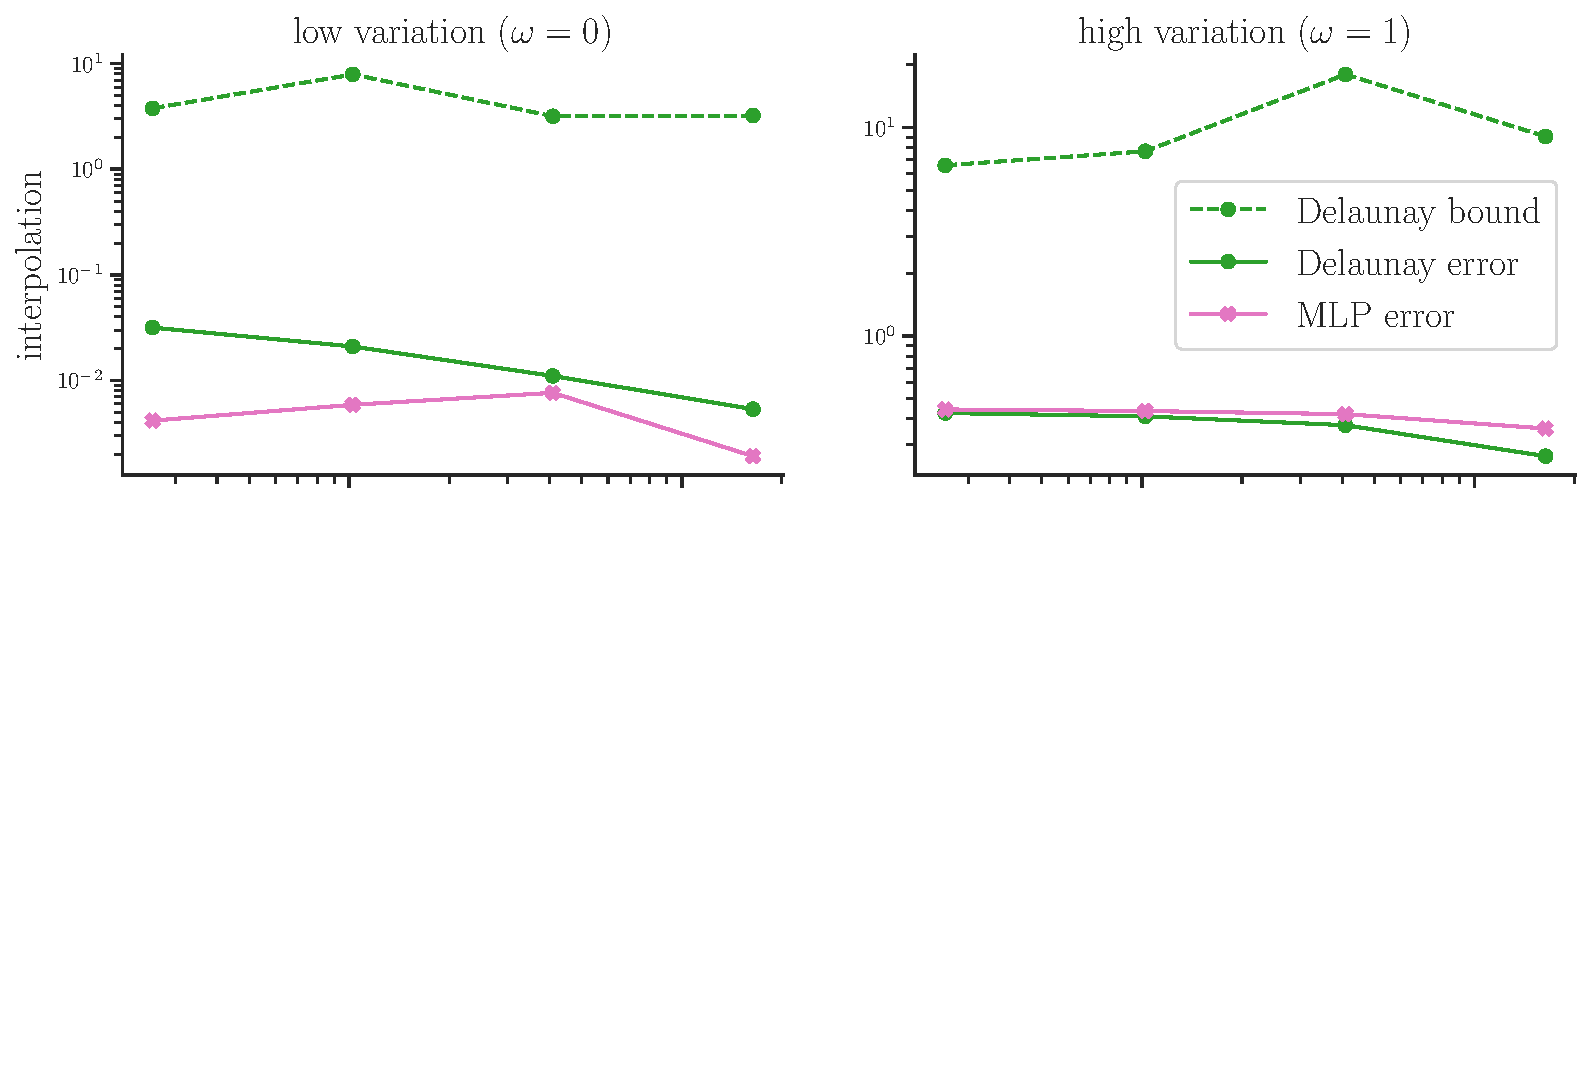
\includegraphics[width=0.75\textwidth]
    {../img/delaunay_new/del_mlp_n_smooth_interp.pdf}\\

    % RBF/GP figure
    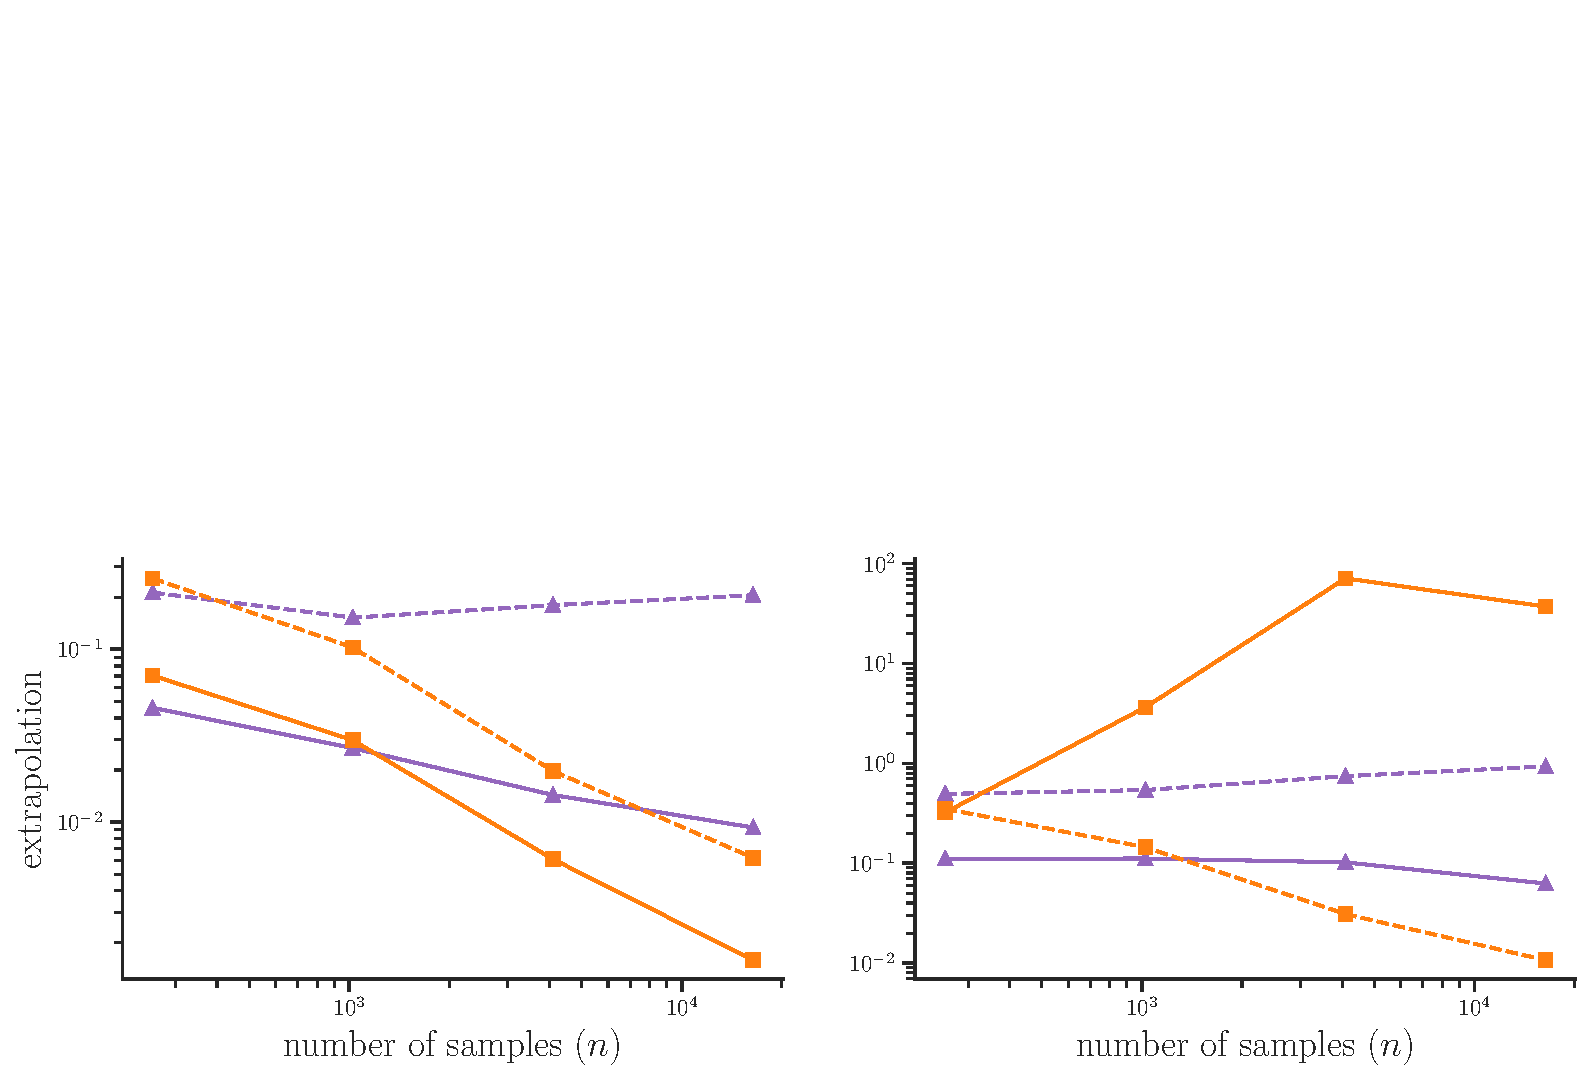
\includegraphics[width=0.75\textwidth]
    {../img/delaunay_new/rbf_gp_n_smooth_extrap.pdf}
    \llap{%
        \raisebox{0.22in}{
        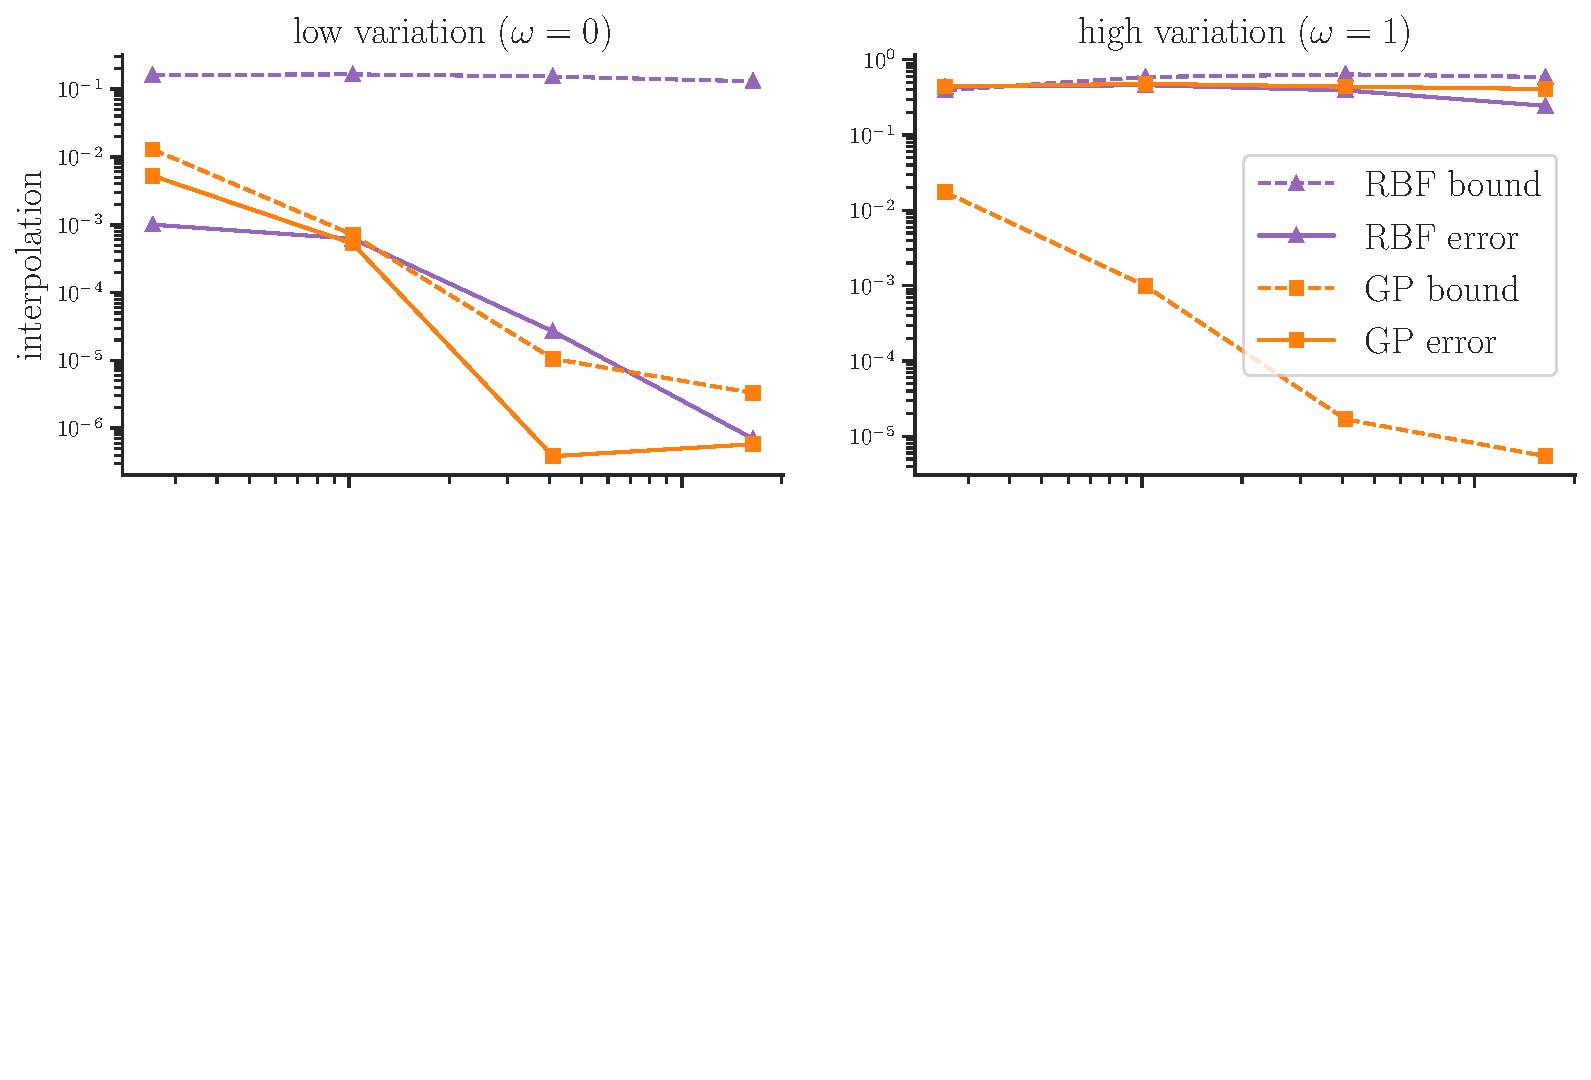
\includegraphics[width=0.75\textwidth]
        {../img/delaunay_new/rbf_gp_n_smooth_interp.pdf}
        }%
    }
    \end{center}
\end{frame}

\section{Experiments on Airfoil SciML Problem}

% Slide 9: Problem definition and experiment
\begin{frame}
\frametitle{Experiments on UIUC Airfoil Dataset}
    {\bf Training set:}\\

    $\sim$1600 labeled images:
    $\qquad f\big($
    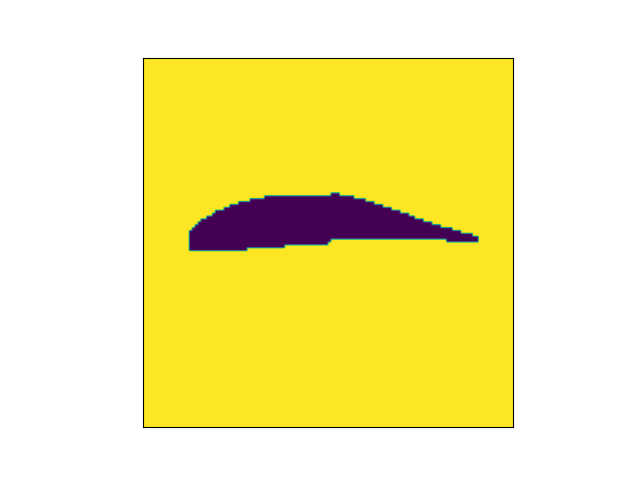
\includegraphics[height=4em]{../img/probs/uiuc_airfoil/test_pt149_0.png}
    $\big) \rightarrow $
    lift/drag

    \bigskip

    {\bf Problem representation:}\\

    % Tikz image of our architecture
    \begin{center}
    {\small
    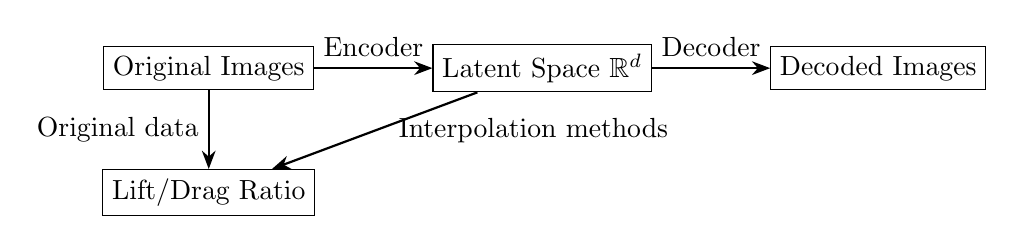
\begin{tikzpicture}[
        node distance=1cm and 1.5cm,
        every node/.style={
            draw, minimum width=1.5cm, minimum height=0.5cm, align=center
        },
        arrow/.style={-Stealth, thick}
    ]
    % Nodes in the top row
    \node (original) {Original Images};
    \node (encoded) [right=of original] {Latent Space $\mathbb{R}^d$};
    \node (decoded) [right=of encoded] {Decoded Images};
    % Nodes in the bottom row
    \node (lift_drag) [below=of original] {Lift/Drag Ratio};
    % Arrows in the top row
    \draw[arrow] (original) -- node[above, draw=none, fill=none]
        {Encoder} (encoded);
    \draw[arrow] (encoded) -- node[above, draw=none, fill=none]
        {Decoder} (decoded);
    % Arrows to the bottom row without boxes around labels
    \draw[arrow] (original) -- node[left, draw=none]
        {Original data} (lift_drag);
    \draw[arrow] (encoded) -- node[right, xshift=5pt, draw=none]
        {Interpolation methods} (lift_drag);
    \end{tikzpicture}
    }
    \end{center}
    \vfill
    \url{https://github.com/ziliHarvey/CNN-for-Airfoil}
\end{frame}

% Slide 10: Results on validation set
\begin{frame}
\frametitle{Results on Validation Set}
    \begin{center}
    \begin{figure}
    \begin{subfigure}{0.55\textwidth}
        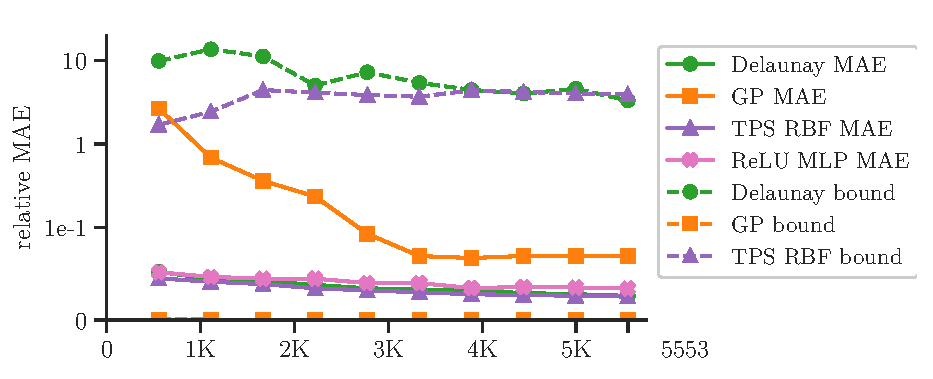
\includegraphics[width=0.8\textwidth]
        {../img/probs/uiuc_airfoil/airfoil_latent4D_error_summary.eps}\\
        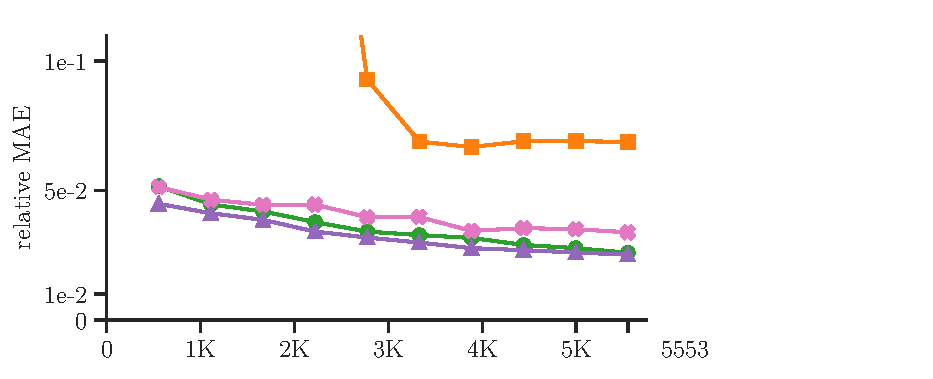
\includegraphics[width=0.8\textwidth]
        {../img/probs/uiuc_airfoil/airfoil_latent4D_error_summary_zoom.eps}
    \end{subfigure}
    \begin{subfigure}{0.43\textwidth}
        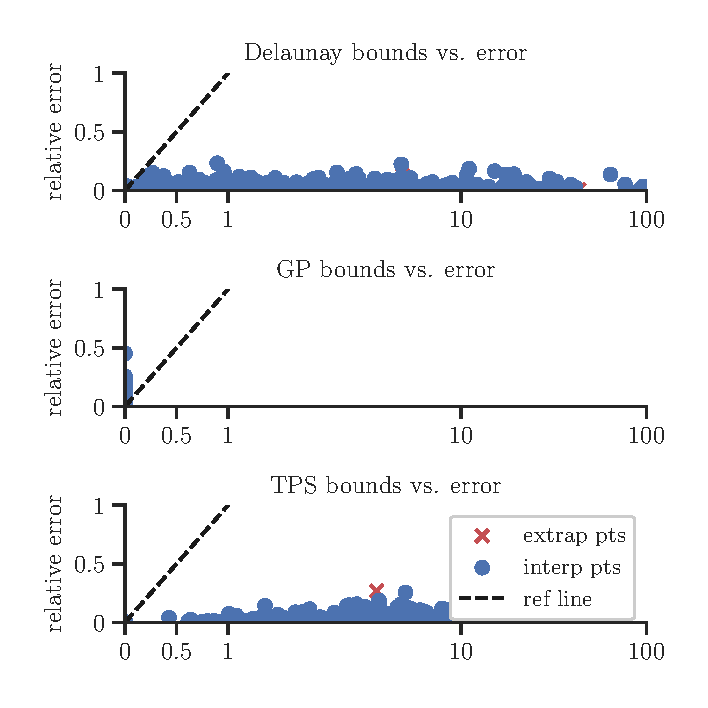
\includegraphics[width=0.8\textwidth]
        {../img/probs/uiuc_airfoil/airfoil_latent4D_scatter.eps}
    \end{subfigure}
    \end{figure}
    \end{center}
\end{frame}

% Slide 11: Results on holdout set

% Slide 12: Conclusion

% Funding acknowledgement
\begin{frame}
\frametitle{Acknowledgements}
    This work was performed under the auspices of the U.S. Department of Energy
    by Lawrence Livermore National Laboratory under Contract DE–AC52–07NA27344
    and the LLNL-LDRD Program under Project tracking No. 21–ERD–028. Release
    number LLNL–JRNL–846568.

    \bigskip

    This work was also supported in part by FASTMath Institute: U.S.~Department
    of Energy, Office of Science, Office of Advanced Scientific Computing
    Research, SciDAC program under contract number DE-AC02-06CH11357 and by
    award DOE–FOA–2493.
\end{frame}

% Final slide
\begin{frame}
\frametitle{Questions}
    \tableofcontents

    \bigskip

    
\includegraphics[width=0.05\textwidth]{../img/logos/logo-gh.png}
    $\quad$
    \url{github.com/LLNL/interpML}

    \bigskip

    {\small
    Chang, Gillette, and Maulik (2025). Leveraging interpolation models and
    error bounds for verifiable scientific machine learning. Journal of
    Computational Physics 524, Article 113726.
    \url{doi.org/10.1016/j.jcp.2025.113726}
    }
\end{frame}

\end{document}
